\lysh{36892}{2}

\begin{alist}
\item Έχουμε ισοδύναμα:
\begin{align*}
\dfrac{|x|}{3} - \dfrac{|x| + 4}{5} &= \dfrac{2}{3} \overset{(\cdot 15)}{\Leftrightarrow} \\
5|x| - 3(|x| + 4) &= 10\text{, οπότε} \\
5|x| - 3|x| - 12 &= 10\text{, δηλαδή} \\
2|x| &= 22\text{, οπότε} \\
|x| &= 11\Leftrightarrow x = -11 \text{ ή } x = 11.
\end{align*}

\item Το τριώνυμο $-x^2 + 2x + 3$ έχει διακρίνουσα $\Delta = \beta^2 - 4\alpha\gamma = 2^2 - 4 \cdot (-1) \cdot 3 = 16 > 0$ και ρίζες τις:
\begin{gather*}
x_1 = \dfrac{-\beta - \sqrt{\Delta}}{2\alpha} = \dfrac{-2 - 4}{2 \cdot (-1)} = 3\text{και} \\
x_2 = \dfrac{-\beta + \sqrt{\Delta}}{2\alpha} = \dfrac{-2 + 4}{2 \cdot (-1)} = -1.
\end{gather*}

Από τον παρακάτω πίνακα προσήμου, βλέπουμε ότι η ανίσωση $-x^2 + 2x + 3 \le 0$ αληθεύει για $x \le -1 \text{ ή } x \ge 3$.

\begin{center}
\begin{tikzpicture}
\tikzset{t style/.style = {style = dashed}}
\tkzTabInit[color,lgt=3,espcl=2,colorC = maincolor!40,
colorL = maincolor!20,
colorV = maincolor!40]%
{$x$ / .8,$-x^2+2x+3$ /0.8}%
{$-\infty$,$-\dfrac{1}{2}$,$1$,$+\infty$}%
\tkzTabLine{ , $-$, z
, $+$ , z
, $-$ , }
\end{tikzpicture}
\end{center}

\item Οι λύσεις της εξίσωσης του $\alpha)$ ερωτήματος είναι και λύσεις της ανίσωσης του $\beta)$ ερωτήματος, διότι $-11 \in (-\infty, -1]$ και $11 \in [3, +\infty)$.
\end{alist}
